\section{Results}

\subsection{DCT Basis Images}

To get the basis function shown in figure 8-1 we can compute an array for each
value of u by sweeping x from 0 to n-1. And in our case, n is equal to the array
length, 8. You can find the source code in the appendix.

\begin{figure}[H]
    \centering
    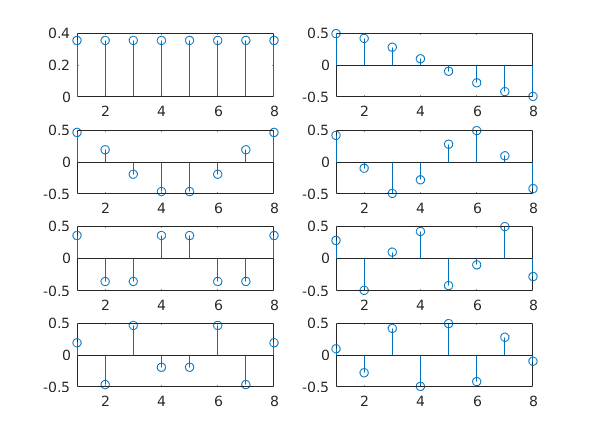
\includegraphics{dct_basis_1d.png}
    \caption{Replicate of figure 8-1}
\end{figure}

The basis functions can be shown to be orthogonal by determining the dot product
between any two of them, which will be zero. I have written a script to
calculate the dot product between each of the above basis functions. The script
can be found in the appendix, the result is contained within an array:

\begin{figure}[H]
    \centering
    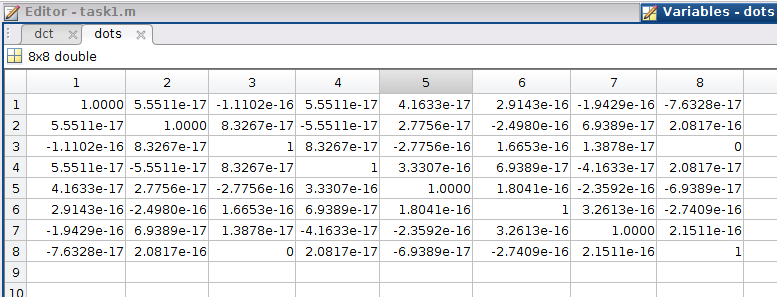
\includegraphics[scale=0.5]{dot.png}
    \caption{Dot products}
\end{figure}

As you can see, many of the dot products are not zero, I am assuming that there
is some sort of rounding or quantization error there as these numbers are
extremely small, to the power of -16 or -17. You will also notice that the dot
product of a basis function with itself is found to be 1. This makes sense as it
must be non-orthogonal to itself.

\subsection{2D DCT Basis Images}

Now to write code to calculate 2D basis images. I will employ our 1D function
from above. Here is the results for 8x8 basis images:

\begin{figure}[H]
    \centering
    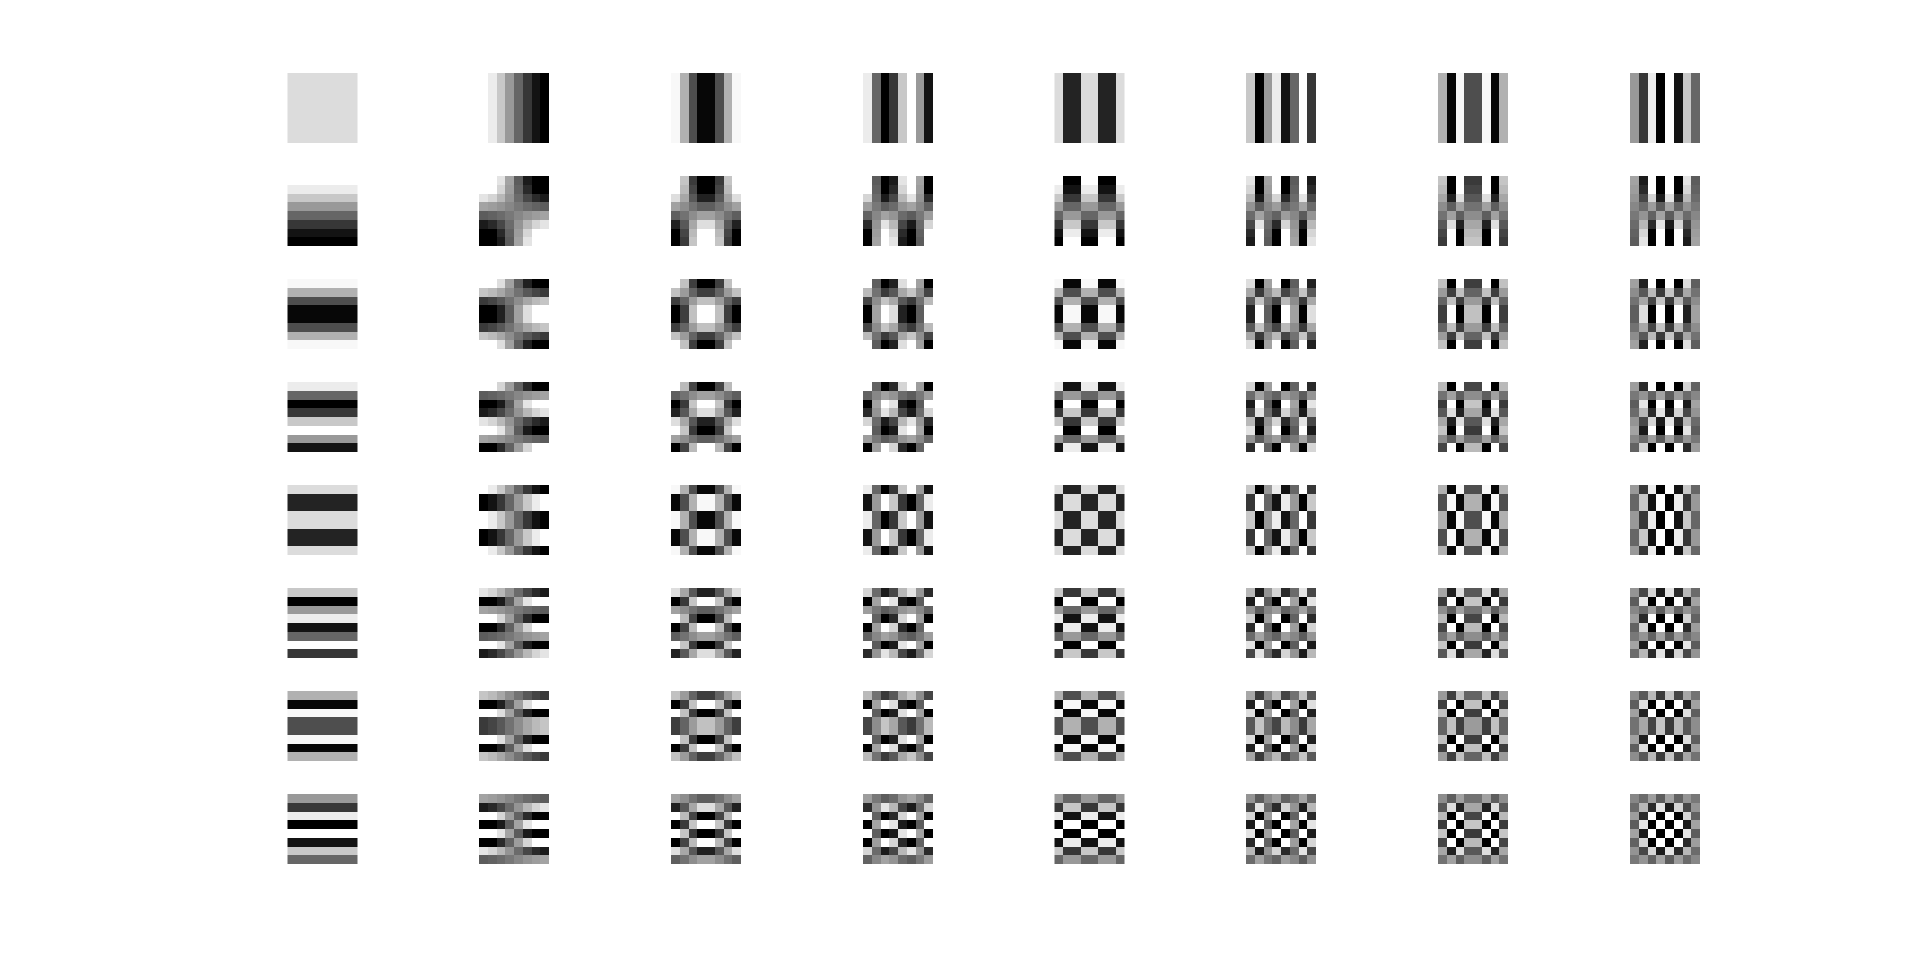
\includegraphics[scale=0.3]{dct2.png}
    \caption{2D DCT Basis Images}
\end{figure}

Each of these small basis images shows the permutations of each frequency
combined in the x axis with every frequency in the y axis. You can observe that
the images on the top row and leftmost column have frequencies in only one
direction and frequencies are equal down the diagonal.
